
\subsection{Debiasing Results}
\tabref{t:templates1} gives results on OCCTMP. Two OCCTMP
examples are given in \tabref{t:templates2}. We see that
DensRay can mitigate the gender bias in BERT as measured by
diff: bias between predicting he/she drops by large margin
(e.g., for bert-base from 1.98 to 0.36). The table indicates
that DensRay outperforms the other two methods on OCCTMP.
Note that
the prediction probabilities of debiasing conceptor are
quite low for both ``he'' and ``she'' indicating that conceptor debiasing might affect language model performance. However,
in relative terms, ``he'' is still strongly favored compared
to ``she''.
\tabref{t:weat1} shows the results on association tests. We observe that association tests have a high variance depending on which category is used. 
Overall the debiasing performance of the three methods are comparable with DensRay and Conceptor having the best performance three times and hard-debiasing having the best performance 5 times.
Overall the debiasing performance of the three methods are comparable, with DensRay and Conceptor both having the best performance three times and hard-debiasing having the best performance 5 times.

\begin{table}[ht]
\centering
\footnotesize
\vspace{0cm}  
\setlength{\abovecaptionskip}{0.2cm}   
\setlength{\belowcaptionskip}{0cm}
\begin{tabular}{lccccc}
\hline
model & prob(he) & prob(she) & sum &diff & var\\
\hline
bert-base & 0.66 & 0.19 & 0.85 &1.98&1.39\\
bert-base-hard & 0.35 & 0.42 & 0.77&0.42&0.09\\
bert-base-conceptor & 0.18 & 0.11 & 0.28 & 0.68&0.26\\
bert-base-densray & 0.48 & 0.37 & 0.86&\textbf{0.36}&0.07\\
\hline
bert-large  & 0.63 & 0.19 & 0.82  &1.82&1.30\\
bert-large-hard & 0.40 & 0.23 & 0.63&0.69&0.30\\
bert-large-conceptor & 0.43 & 0.18 & 0.61 & 1.03&0.53\\
bert-large-densray  & 0.47 & 0.31 & 0.77&\textbf{0.49}&0.13 \\
\hline
\end{tabular}
\caption{\tablabel{t:templates1} BERT debiasing results on OCCTMP. \textit{bert-base} and \textit{bert-large} are the original models without debiasing. \textit{prob(he)} is
	the average probability predicted for \textit{he} as the [MASK] in OCCTMP. We also show the average sum probability $sum=prob(he)+prob(she)$ which we take as an indication of 
	language model performance and \textit{var}, the variance of \textit{ diff}, for reference.}
\end{table}

\begin{table}[h]
	\centering
	\footnotesize
	\vspace{0cm}  
	\setlength{\abovecaptionskip}{0.2cm}   
	\setlength{\belowcaptionskip}{0cm}
	\begin{tabular}{cl{|}cccc{|}cccc}
		\hline
		&&\multicolumn{4}{c|}{bert-base}&\multicolumn{4}{c}{bert-large}\\
		%\hline
		&&\multicolumn{2}{c}{WEAT}&\multicolumn{2}{c|}{SEAT}&\multicolumn{2}{c}{WEAT}&\multicolumn{2}{c}{SEAT}\\
		\hline
		category & model & d & p& d & p& d & p& d & p\\
		\hline
		C6 & without debiasing & 0.66 & 0.08 &1.04&$<$10$^{-2*}$& 1.57 & $<$10$^{-2*}$ &0.50&$<$10$^{-2*}$\\
		& hard debiasing& 0.15 & 0.38&\textbf{-0.08}&0.67& 0.80 & 0.06&0.07&0.35\\
		& debiasing conceptor & \textbf{0.07} & 0.46&0.77&$<$10$^{-2*}$ & 1.33 & $<$10$^{-2*}$&\textbf{0.06}&0.37\\
		&densray & 0.62 & 0.12&0.36&0.02$^{*}$ & \textbf{0.76} & 0.07&0.13&0.22\\
		\hline
		C7 & without debiasing & 0.60 & 0.11 &0.17&0.15 & -0.40 & 0.75 &0.38&0.01$^{*}$\\
		& hard debiasing & \textbf{-0.07} & 0.56&\textbf{-0.06}&0.64 & -0.51 & 0.83&0.38&0.01$^{*}$\\
		& debiasing conceptor & 0.54 & 0.14&-0.25&0.93 & -0.32 & 0.73&\textbf{-0.60}&0.99\\
		& densray & 0.09 & 0.45&-0.47&0.99 & \textbf{0.06} & 0.05&-0.73&0.99\\
		\hline
		C8& without debiasing & 0.78 & 0.08 &0.81&$<$10$^{-2*}$ & -0.60 & 0.87 &-0.30&0.95\\
		& hard debiasing & -0.29 & 0.68&\textbf{-0.10}&0.71 & 0.78 & 0.06&\textbf{-0.03}&0.56\\
		& debiasing conceptor & 0.62 & 0.14&0.50&$<$10$^{-2*}$& \textbf{0.12} & 0.39&0.30&0.94\\
		& densray & \textbf{0.03} & 0.47&0.41&0.01$^{*}$ & 0.20 & 0.33&-0.66&0.99\\
		\hline
	\end{tabular}
	\caption{\tablabel{t:weat1}
		BERT debiasing results on association tests. * shows significant gender bias. Only models without significant gender bias ($p>0.05$) can be accepted.}
\end{table}

\subsection{Model Performance}
\tabref{t:glue1} shows that DensRay debiasing gets comparable results with
the original models on Wikitext-2 and GLUE tasks.
In most tasks on bert-base and all tasks on bert-large, DensRay performs better than hard debiasing, so DensRay affects model performance less.
Similarly, in most tasks on bert-base and all tasks but one
on bert-large, DensRay performs better than debiasing conceptor. Overall we find that DensRay affects model performance the least among the considered methods.
\begin{table*}[h]
\centering
\footnotesize
\vspace{0cm}  
\setlength{\abovecaptionskip}{0.2cm}   
\setlength{\belowcaptionskip}{0cm}
\begin{tabular}{l||c|cccccccccc}
%\hline
model & Wikitext-2&CoLA &SST-2&MRPC&STS-B&RTE&WNLI&GLUE avg\\
\hline\hline
		bert-base &3.77&49.15&92.09&85.86&82.66&62.82&52.11&70.78\\
bert-base-hard &3.95&45.53&\textbf{91.74}&82.48&\textbf{82.60}&63.54&\textbf{56.34}&70.37\\
bert-base-conceptor &4.46&\textbf{48.31}&91.43&84.08&81.37&59.57&\textbf{56.34}&70.18\\
bert-base-densray &\textbf{3.81}&48.04&\textbf{91.74}&\textbf{84.89}&82.43&\textbf{63.90}&53.52&\textbf{70.75}\\
\hline
bert-large &3.29& 47.93&94.90&89.30&87.60&70.10&65.10&75.82\\
bert-large-hard &3.85& 47.45&93.95&85.01&82.33&67.12&63.02&73.15\\
bert-large-conceptor &4.13&\textbf{49.44}&93.87&87.67&83.44&62.45&56.34&72.20\\
bert-large-densray &\textbf{3.35}& 48.91&\textbf{94.02}&\textbf{88.84}&\textbf{85.63}&\textbf{67.78}&\textbf{64.48}&\textbf{74.94}\\
%\hline
\end{tabular}
\caption{\tablabel{t:glue1}
Language modeling perplexity and GLUE tasks
performance. }
\end{table*}


\subsection{Examples}
In \tabref{t:templates2} we show two OCCTMP examples.
Again, densray works best as measures by diff.
The sum probabilities of ``he'' and ``she''
on the debiasing conceptor are around 0.5, indicating that
the language model has lost part of its ability to predict that 
a pronoun is  likely to occur in the masked position.
\begin{table}[h]
	\centering
	\footnotesize
		\vspace{0cm}  
	\setlength{\abovecaptionskip}{0.2cm}   
	\setlength{\belowcaptionskip}{0cm}  
	\begin{tabular}{llcccc}
		\hline
		sentence & model & prob(he) & prob(she) &sum&diff\\
		\hline
		[MASK] is a & bert-base & 0.84 & 0.13&0.97&1.86\\
		professor.& bert-base-hard& 0.37 & 0.55&0.92&0.40\\
		& bert-base-conceptor& 0.28 & 0.23&0.51&{0.20}\\
		& bert-base-densray & 0.53 & 0.37&0.90&0.36\\
		\hline
		[MASK] is a & bert-base & 0.22 & 0.72&0.94&1.19\\
		dancer.  & bert-base-hard& 0.27 & 0.64&0.91&0.86\\
		& bert-base-conceptor& 0.20 & 0.33&0.53&0.50\\
		& bert-base-densray& 0.42 & 0.52&0.94&0.21\\
		\hline
	\end{tabular}
	\caption{\tablabel{t:templates2}
		OCCTMP examples with prediction probabilities.}
\end{table}

\subsection{Analysis}

\subsubsection*{Debiasing on Attention Heads and Layers}
We now apply DensRay to single attention heads in BERT and investigate the debiasing effect on OCCTMP. The heatmap \figref{fig:heads} shows that the debiasing effect of one single attention head is not apparent, with diff scores all in (1.0,1.4). We conclude that there is no single attention head that is responsible for processing gender information.
This conclusion is similar to the experiment from \newcite{bau2019identifying}, which showed modifying some neurons activations in NMT didn't help in controlling gender, and conjectured that gender property is very distributed on the neurons.

So far we have always applied DensRay to all BERT layers
simultaneously. \figref{fig:layersbase}  illustrates the effect of
debiasing a single  layer on our templates and the three
WEAT categories.  In contrast to the attention heads we observe a different debiasing effect across different layers. We see that the debiasing effect is
stronger in layers 7--10 than in the other layers in
bert-base. It is shown that gender information is processed on BERT layers, especially the upper layers.
\begin{figure}[h]
	\centering
	\footnotesize
	\subfigure[attention heads]{
		\begin{minipage}[l]{0.5\linewidth}
			\centering
			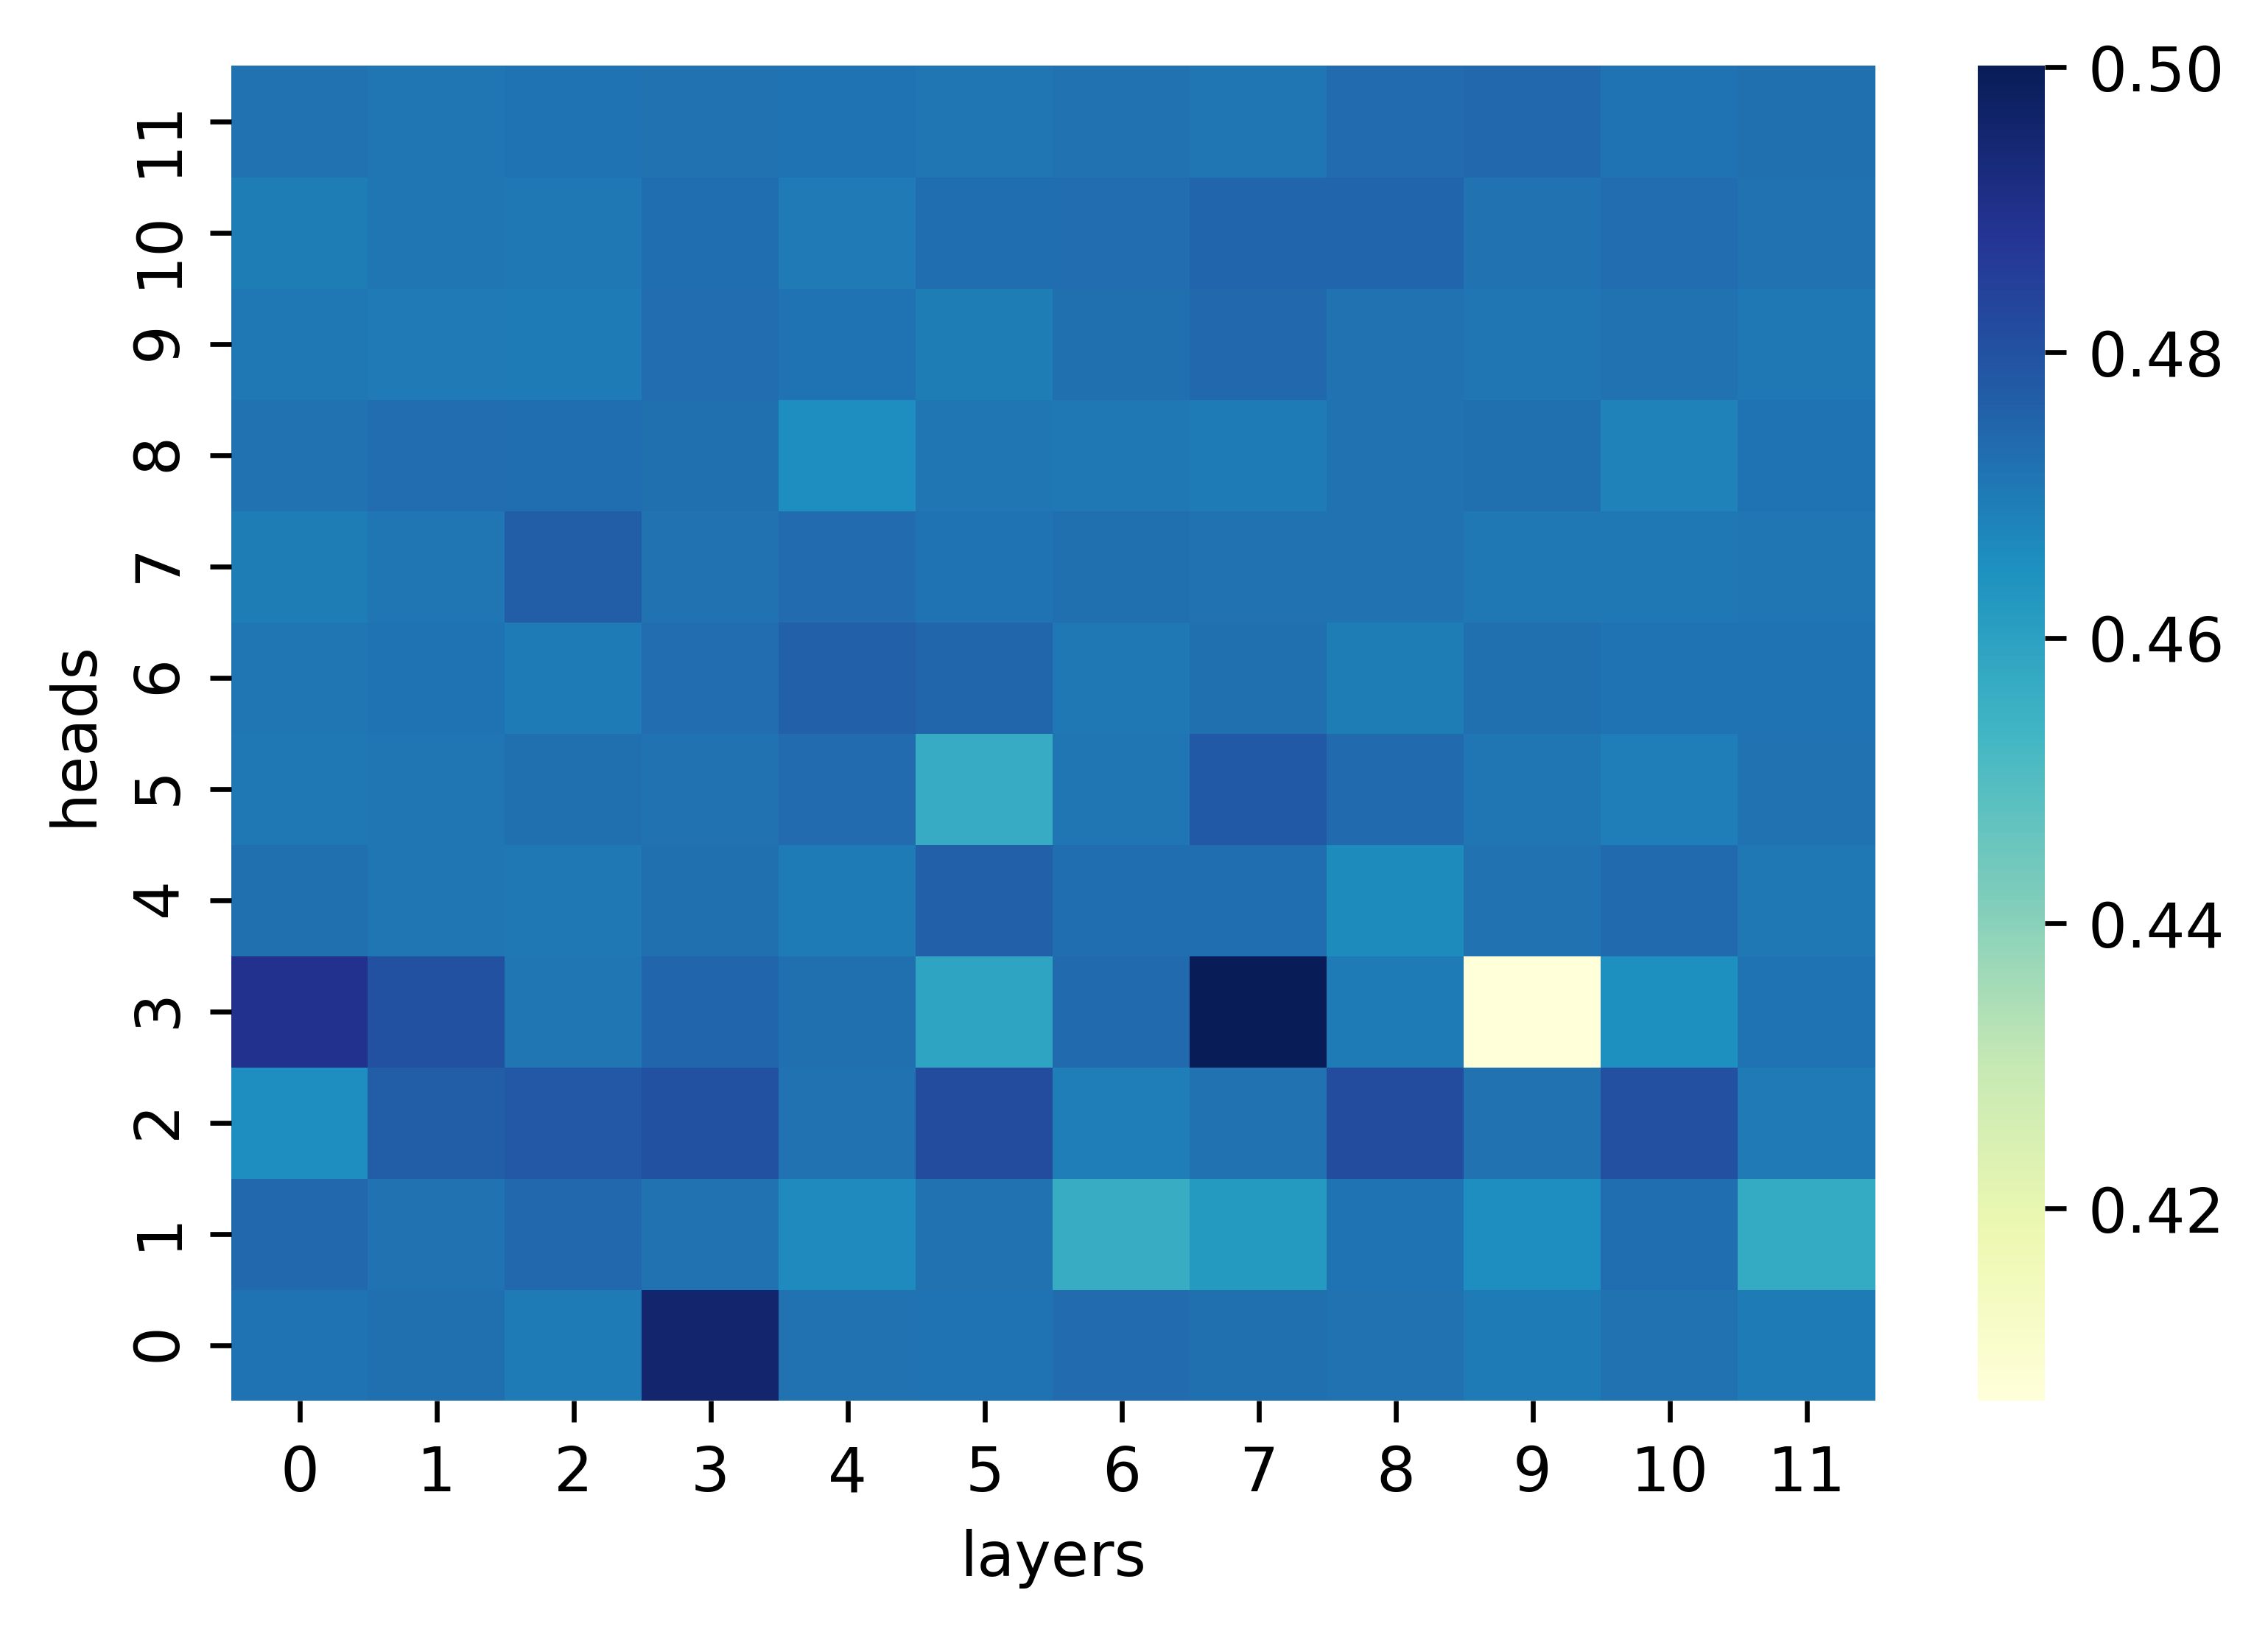
\includegraphics[width=0.75\linewidth]{heads}
			\figlabel{fig:heads}
		\end{minipage}%
	}%
	\subfigure[layers]{
		\begin{minipage}[r]{0.5\linewidth}
			\centering
			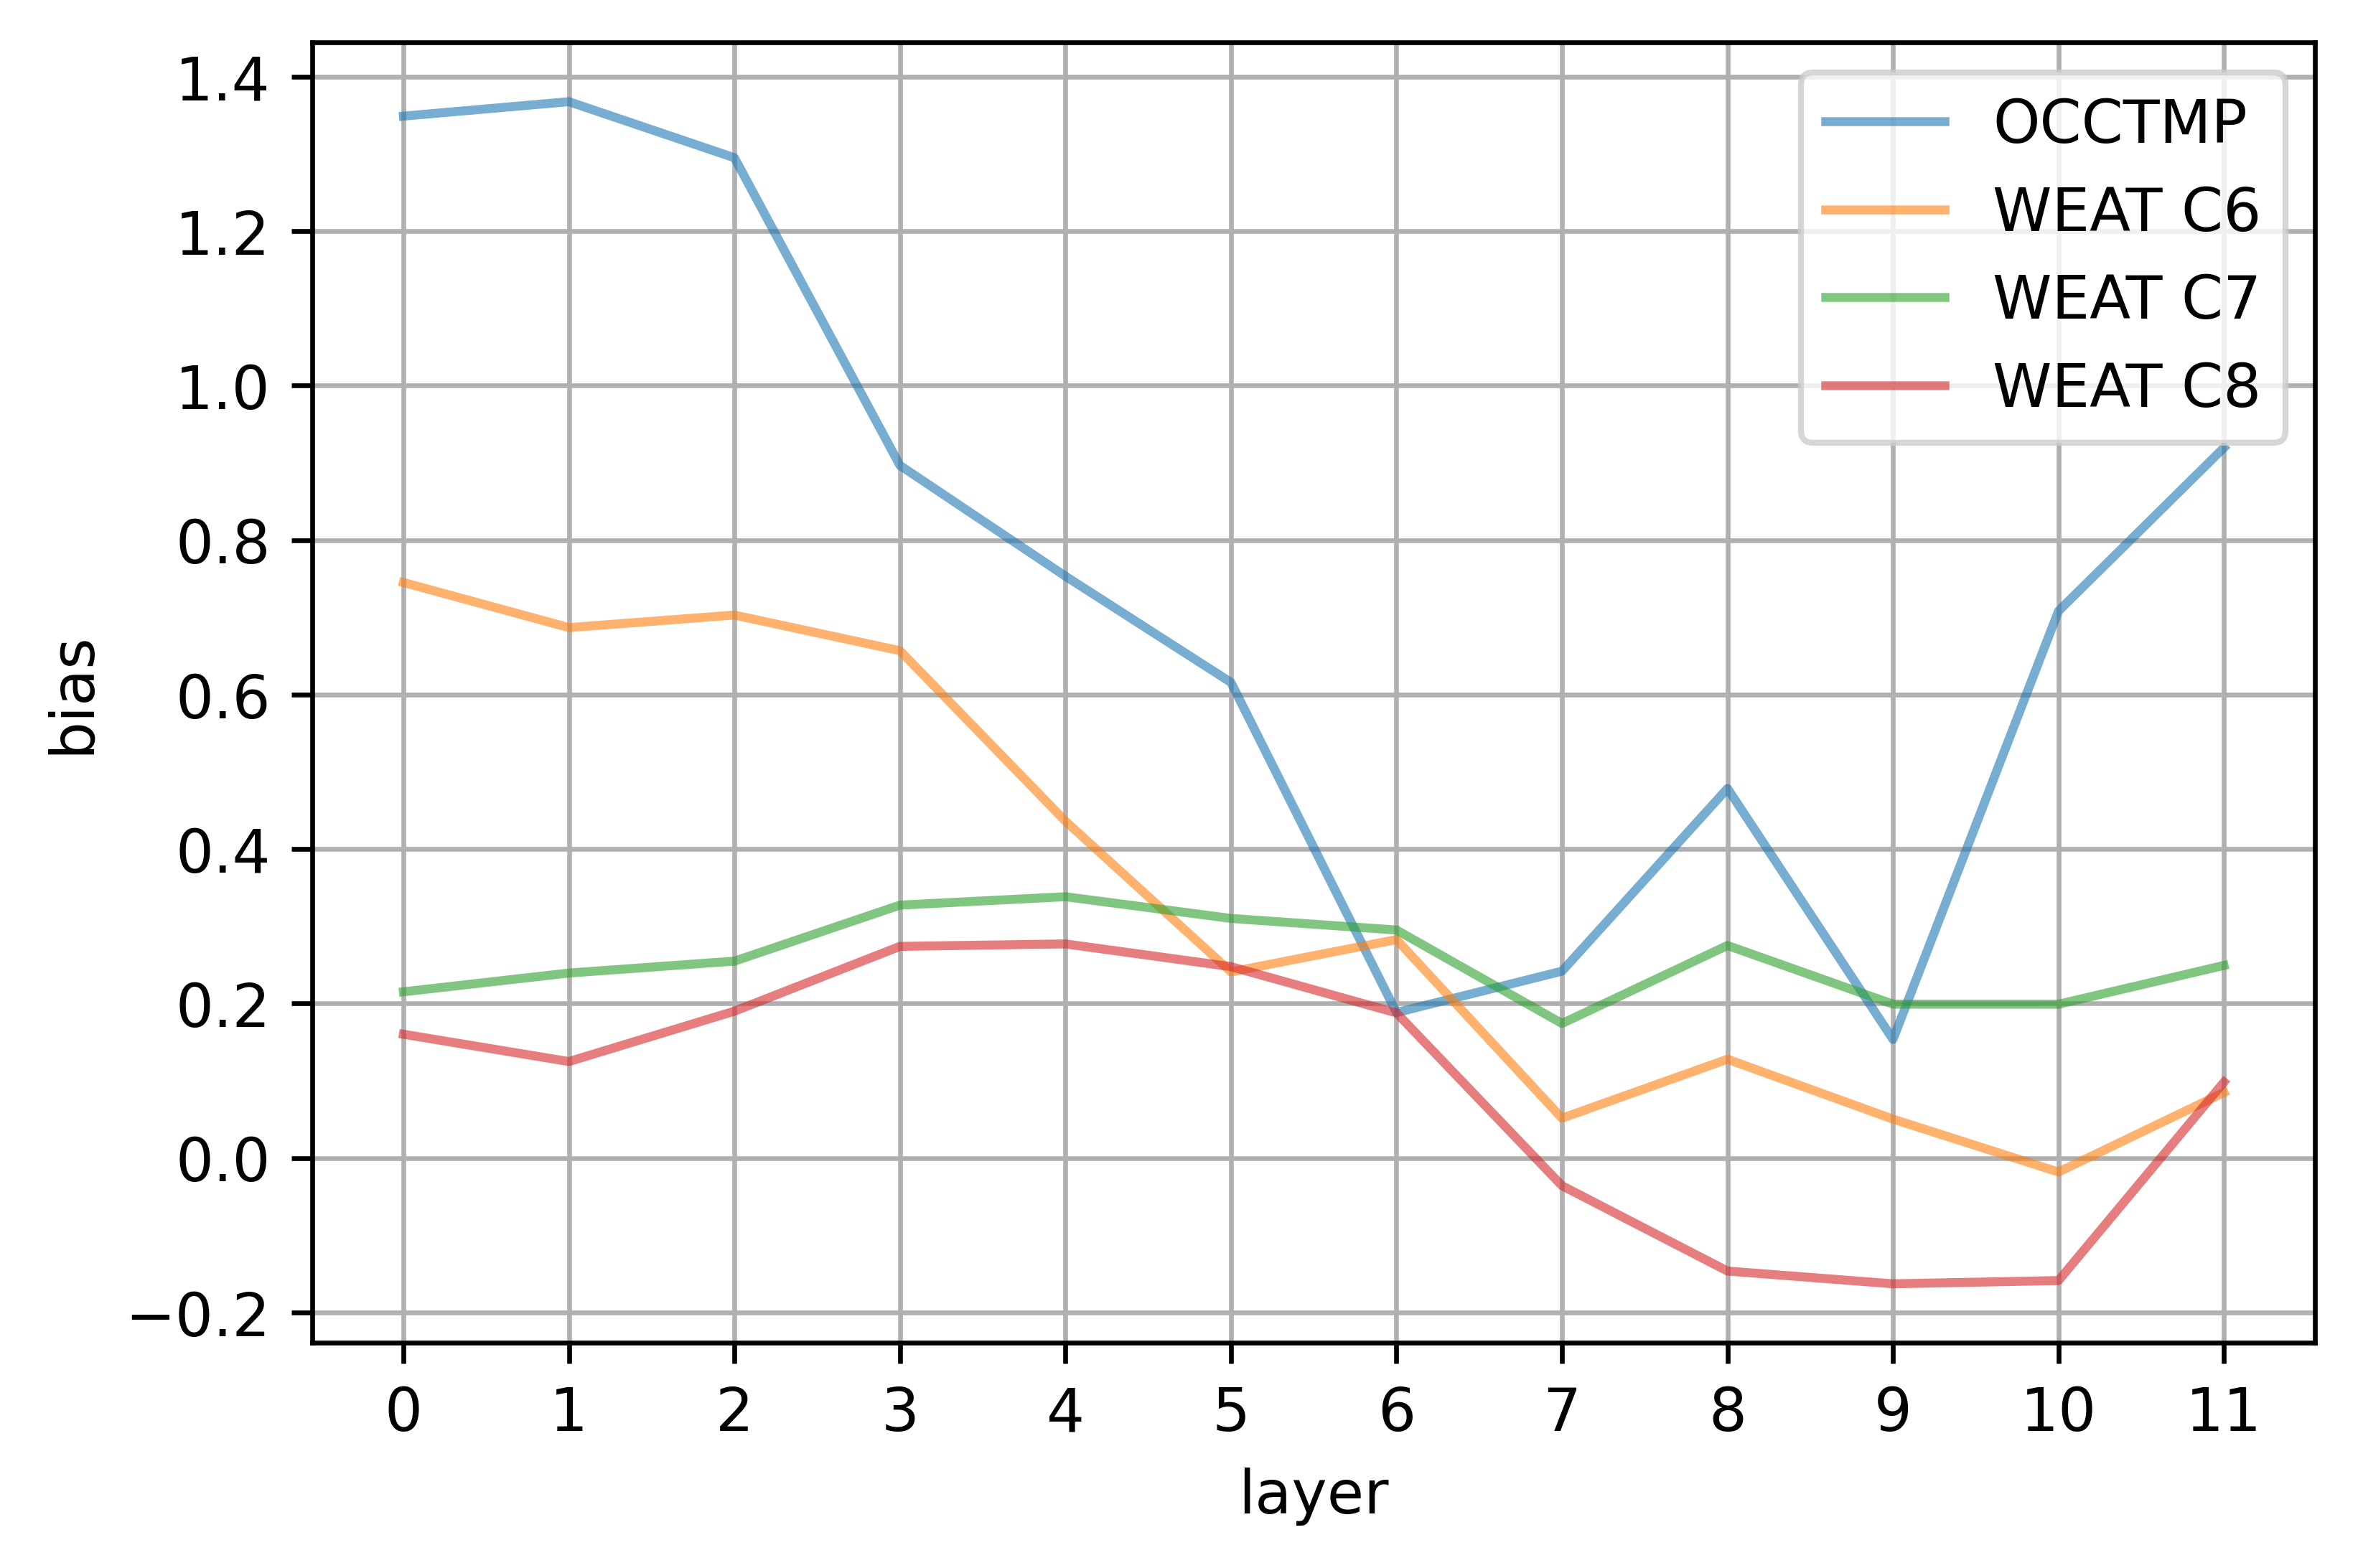
\includegraphics[width=0.75\linewidth]{layers}
			\figlabel{fig:layersbase}
		\end{minipage}%
	}%
	\centering
	\caption{(a): DensRay debiasing on each single attention head in bert-base, measured by \text{diff} on OCCTMP. (b): DensRay debiasing on each single layer, measured by \text{diff} on  OCCTMP and $d$-value on WEAT.}
	\figlabel{fig:headsandlayers}
\end{figure}

\subsubsection*{Quantifying Gender Bias with DensRay}
\seclabel{quantify}
DensRay can be used to quantify gender bias for sentences
and tokens. We use the distance to the origin in the gender
subspace as the measure. In BERT, we use the average
bias score of tokens to quantify the whole
sentence. \tabref{t:measure1} compares DensRay with the log
probability score \cite{kurita2019measuring}, which
quantifies gender bias based on templates of form ``[TARGET]
is a [ATTRIBUTE]''. We regard zero as a balance point
without bias. Contrary to the log probability score, a
positive DensRay score represents the level of female
bias. These examples show that DensRay is more versatile, it
can quantify  bias both on the token and on the sentence level in contrast to the log-probability score.
In the sentence ``The professor asked the nurse .'' one can immediately see that the model has a male bias on ``professor'' and a female bias on ``nurse'', although the sentence itself
is completely gender-neutral.

\begin{table}[h]
	\centering
	\footnotesize
	\vspace{0cm}  
	\setlength{\abovecaptionskip}{0.2cm}   
	\setlength{\belowcaptionskip}{0cm}
	\begin{tabular}{cccccc|c||c}
		\hline
		\multicolumn{6}{c|}{DensRay}&Avg.&log probability score\\		
		\hline\hline
		[MASK] &is &a &professor& . &&&\\
		-0.69 &-0.97 &-0.9  &-0.15  &0.45& &-0.45& 0.63\\
		\hline
		[MASK] &is &a &nurse& . &&&\\
		2.43  &1.34  &1.7   &1.93  &0.5&& 1.58 &-5.44\\
		\hline
		The &professor &asked &me& . &&&\\
		-1.25 &-0.55 &-0.08  &0.59  &0.35 &&-0.19 &
                not applicable\\
		\hline
		The &professor &asked &the&nurse &.&&\\
		-1.3&  -0.25  &0.24  &1.28  &2.19
                &0.45&0.43& not applicable\\
		\hline
	\end{tabular}
	\caption{\tablabel{t:measure1}
		Examples for quantifying bias (model: bert-base).}
\end{table}




\subsubsection*{Alternatives to Removing the Gender Dimension}
In our experiments, we zero out the dimensions of the gender
subspace to remove gender bias. 
We also explored three alternatives to zeroing out. 1)
Replace the first dimension of the gender subspace with the
mean value of the first dimension of the training
samples. 2) Standardize the first dimension. 3) Replace the
first dimension with a small random variable sampled from a Gaussian distribution. All of them did not perform well. Using higher dimensional gender subspaces also did not improve the debiasing results while harming the model performance.


\subsection{Multilingual Debiasing}
We now show that, in a multilingual contextualized language model like mBERT, we can use DensRay for zero-shot debiasing. Specifically, we train a DensRay model on English and use it to debias Chinese.

In our opinion, multilingual debiasing involves two distinct
	problems. First, how can bias be removed from the underlying
	model? Second, how does bias manifest in a particular
	language? The removal of bias from the underlying model can
	be argued to be largely independent of the language whereas
	the way bias manifests is highly language-dependent. For
	example, Chinese does not mark gender and most German nouns
	describing people are gender-specific. So on the surface,
	Chinese are gender-neutral and German
	cannot be gender-neutral (e.g. \textit{Studentinnen} and \textit{Studenten}). However, these particularities of surface form of individual
	languages do not change the underlying problem of biased
	language models: Chinese and German language models are
	still biased and should be debiased to avoid unfair and
	biased impact caused by deployed NLP systems.
	
We use  bert-base-multilingual-uncased from
\cite{wolf2019huggingfaces}. We use the same setup as for
bert-base-uncased in our previous experiments. As before, we
compute the rotation matrices using the English gendered
words from the ``family'' category of the Google analogy
test set \cite{mikolov2013efficient}. Since Chinese is a language that does not mark gender, we can construct the OCCTMP templates by directly translating from the English templates. We use the following form:
``\text{[MASK]}\yin{是一个}\textit{occupation}\yin{。}'' We translate the occupation using Tencent Translation\footnote{https://fanyi.qq.com/} and make some manual adjustments to the translation. After removing duplicates,  302 Chinese templates remain.

\tabref{t:templates3} gives results for the Chinese templates. Two examples are given in \tabref{t:templates3}. We see that DensRay trained with English can mitigate gender bias in mBERT: the diff score drops from 1.39 to 1.22 on Chinese templates. 
\begin{table}[h]
	\centering
	\footnotesize
	\vspace{0cm}  
	\setlength{\abovecaptionskip}{0.2cm}   
	\setlength{\belowcaptionskip}{0cm}
	\begin{tabular}{lccccc}
		\hline
		model & prob(he) & prob(she) & sum &diff & var\\
		\hline
		 bert-multi-en 
		& 0.51 & 0.14 & 0.65 & 1.66&0.81 \\ 
		bert-multi-densray-en & 0.33 & 0.12 & 0.46 & 1.33&0.65 \\
		\hline
		 bert-multi-zh 
		& 0.24 & 0.07 & 0.31 & 1.39&0.60 \\
		 bert-multi-densray-zh 
		& 0.12 & 0.04 & 0.17 & 1.22&0.47\\
		\hline
	\end{tabular}
	\caption{\tablabel{t:templates3}
		Results of OCCTMP on mBERT after applied DensRay. Models with \textit{-en} are tested on English templates, and those with \textit{-zh} are tested on Chinese templates.}
\end{table}

\begin{table}[h]
	\centering
	\footnotesize
	\vspace{0cm}  
	\setlength{\abovecaptionskip}{0.2cm}   
	\setlength{\belowcaptionskip}{0cm}
	\begin{tabular}{llcccc}
		\hline
		sentence & model & \yin{prob(他)} & \yin{prob(她)}&sum&diff\\
		\hline
		\yin{\text{[MASK]}是一个客座教授。} & bert-multi-en & 0.68 & 0.16&0.84&1.45\\
		\text{[MASK]} is an adjunct professor.& bert-multi-densray-en & 0.51 & 0.18&0.70&1.04\\
		& bert-multi-zh & 0.52 & 0.11&0.63&1.55\\
		& bert-multi-densray-zh & 0.30 & 0.08&0.38&1.31\\
		\hline
		\yin{\text{[MASK]}是一个管理员。} & bert-multi-en & 0.53 & 0.17&0.70&1.14\\
		\text{[MASK]}is an administrator.& bert-multi-densray-en & 0.35 & 0.13&0.48&0.99\\
		& bert-multi-zh & 0.68 & 0.16&0.84&1.45\\
		& bert-multi-densray-zh & 0.51 & 0.18&0.69&1.04\\
		\hline
	\end{tabular}
	\caption{\label{t:templates3}
		Sanity check on the Chinese templates, where \yin{\textit{他}} means \textit{he} and \yin{\textit{她}} means \textit{she}. Corresponding English translations are shown below the Chinese.}
\end{table}
